%==============================================================================================================
%==============================================================================================================
% Para el grupo de Jefferson
%==============================================================================================================
%==============================================================================================================

Considerando el sistema lineal
$$ Ax=b$$
$$ A=\begin{pmatrix}
     3 &  2 \\
     2 &  6 \\
    \end{pmatrix}\ $$
    
$$ b=\begin{pmatrix}
     2 \\
     -8 \\
    \end{pmatrix}\ $$
    
Escribe la función $ \Phi(x) $ y muestre una interpretación gráfica de la solución de dicho sistema lineal. Pruebe algunas iteraciones del Método del Gradiente después de probar su convergencia.\\

\textbf{Solución:}

El Método del Gradiente converge para el caso debido a que es una matriz simétrica positiva. Esto es porque sus autovalores son positivos ($ \lambda _1 = 2$, $\lambda _2 = 7$).

Considerando un valor inicial 
$$x_0 = \begin{pmatrix}
     15 \\
     -13 \\
    \end{pmatrix}\ $$
Podemos mostrar en la siguiente tabla los valores del los vectores en cada iteración

\begin{table}[h]
    \centering
    \begin{tabular}{r|l|l}
        Iteración & $x$ &    $y$   \\
        \hline
         0  &  15  &  -13 \\
         1  &  10.8548 & -3.2465 \\
         2  &  5.9412 & -5.3348 \\
         3  &  4.6845 & -2.3779 \\
         4  &  3.1948 & -3.0110 \\
         5  &  2.8138 & -2.1146 \\
         6  &  2.3622 & -2.3065 \\
         7  &  2.2467 & -2.0347 \\
         8  &  2.1098 & -2.0929 \\
         9  &  2.0748 & -2.0105 \\
         10  & 2.0333  & -2.0282 \\
         11  & 2.0227  & -2.0032 \\
         12  & 2.0101  & -2.0085 \\
         13  & 2.0069  & -2.0010 \\
         14  & 2.0031  & -2.0026 \\
    \end{tabular}
\end{table}

\begin{center}
    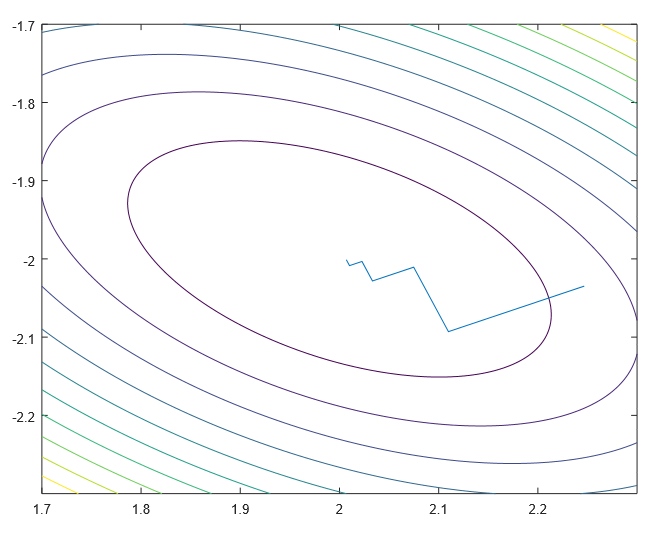
\includegraphics[scale=0.5]{AlfioQuarteroni/Jefferson.png} 
\end{center}

De acuerdo a la gráfica, el Método del Gradiente converge a la solución que está en $(2,-2)$ y es el mínimos de la función cuadrática $\Phi(x)$\\

%==============================================================================================================
%==============================================================================================================
% Para el grupo de Victor
%==============================================================================================================
%==============================================================================================================

Considerando el sistema lineal
$$ Ax=b$$
$$ A=\begin{pmatrix}
     3 &  2 \\
     2 &  6 \\
    \end{pmatrix}\ $$
    
$$ b=\begin{pmatrix}
     2 \\
     -8 \\
    \end{pmatrix}\ $$
    
Escribe la función $ \Phi(x) $ y muestre una interpretación gráfica de la solución de dicho sistema lineal. Pruebe algunas iteraciones del Método del Gradiente después de probar su convergencia.\\

\textbf{Solución:}

El Método del Gradiente converge para el caso debido a que es una matriz simétrica positiva. Esto es porque sus autovalores son positivos ($ \lambda_1=2, \lambda_2=7$).

Considerando un valor inicial 
$$x_0 = \begin{pmatrix}
     15 \\
     -13 \\
    \end{pmatrix}\ $$
Podemos mostrar en la siguiente tabla los valores del los vectores en cada iteración

\begin{table}[h]
    \centering
    \begin{tabular}{r|l|l}
        Iteración & $x$ &    $y$   \\
        \hline
         0  &  -9  &  8 \\
         1  & -6.08562 & -0.51897 \\
         2  &  -1.39448 & 1.08589 \\
         3  & -0.49513 & -1.54297 \\
         4  & 0.95250 & -1.04773 \\
         5  &   1.23003 & -1.85897 \\
         6  & 1.67675 &  -1.70614 \\
         7  & 1.76240 & -1.95648 \\
         8  & 1.90025 & -1.90932 \\
         9  & 1.92668 & -1.98657 \\
         10  & 1.96922 & -1.97202\\
         11  & 1.97737 & -1.99586 \\
         12  & 1.99050 & -1.99136 \\
         13  & 1.99302 & -1.99872 \\
         14  & 1.99707 & -1.99734 \\
    \end{tabular}
\end{table}

\begin{center}
    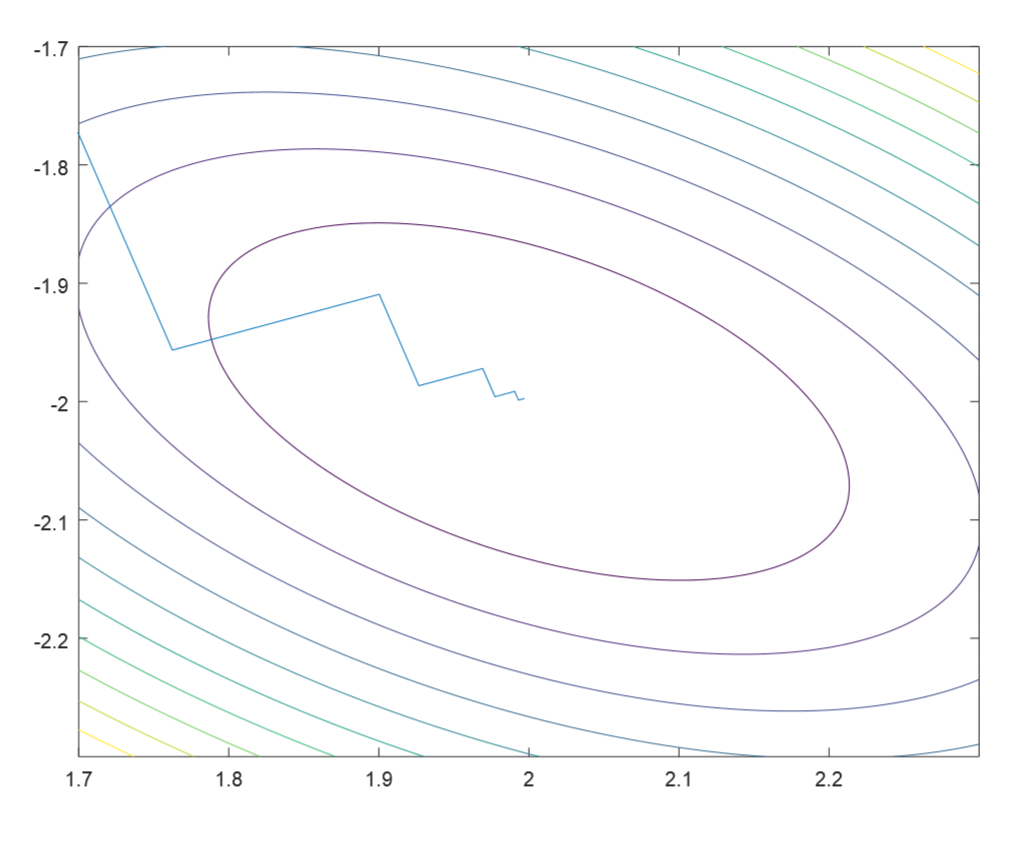
\includegraphics[scale=0.5]{AlfioQuarteroni/Victor.png} 
\end{center}


De acuerdo a la gráfica, el Método del Gradiente converge a la solución que está en $(2,-2)$ y es el mínimos de la función cuadrática $\Phi(x)$\\
%==============================================================================================================
%==============================================================================================================
% Para el grupo de Vittorino
%==============================================================================================================
%==============================================================================================================

Considerando el sistema lineal
$$ Ax=b$$
$$ A=\begin{pmatrix}
     3 &  2 \\
     2 &  6 \\
    \end{pmatrix}\ $$
    
$$ b=\begin{pmatrix}
     2 \\
     -8 \\
    \end{pmatrix}\ $$
    
Escribe la función $ \Phi(x) $ y muestre una interpretación gráfica de la solución de dicho sistema lineal. Pruebe algunas iteraciones del Método del Gradiente después de probar su convergencia.\\

\textbf{Solución:}

El Método del Gradiente converge para el caso debido a que es una matriz simétrica positiva. Esto es porque sus autovalores son positivos ($ \lambda_1=2, \lambda_2=7$).

Considerando un valor inicial 
$$x_0 = \begin{pmatrix}
     15 \\
     -13 \\
    \end{pmatrix}\ $$
Podemos mostrar en la siguiente tabla los valores del los vectores en cada iteración

\begin{table}[h]
    \centering
    \begin{tabular}{|r|l|l|}
        Iteración & $x$ &    $y$   \\
        \hline
         0  &  11  & 4  \\
         1  & 5.3233 & -3.8601 \\
         2  & 2.3889 & -1.7407 \\
         3  & 2.1436 & -2.0804 \\
         4  & 2.0168 & -1.9888 \\
         5  & 2.0062 & -2.0035 \\
         6  & 2.0007 & -1.9995 \\
         7  & 2.0003 & -2.0002\\

    \end{tabular}
\end{table}

\begin{center}
    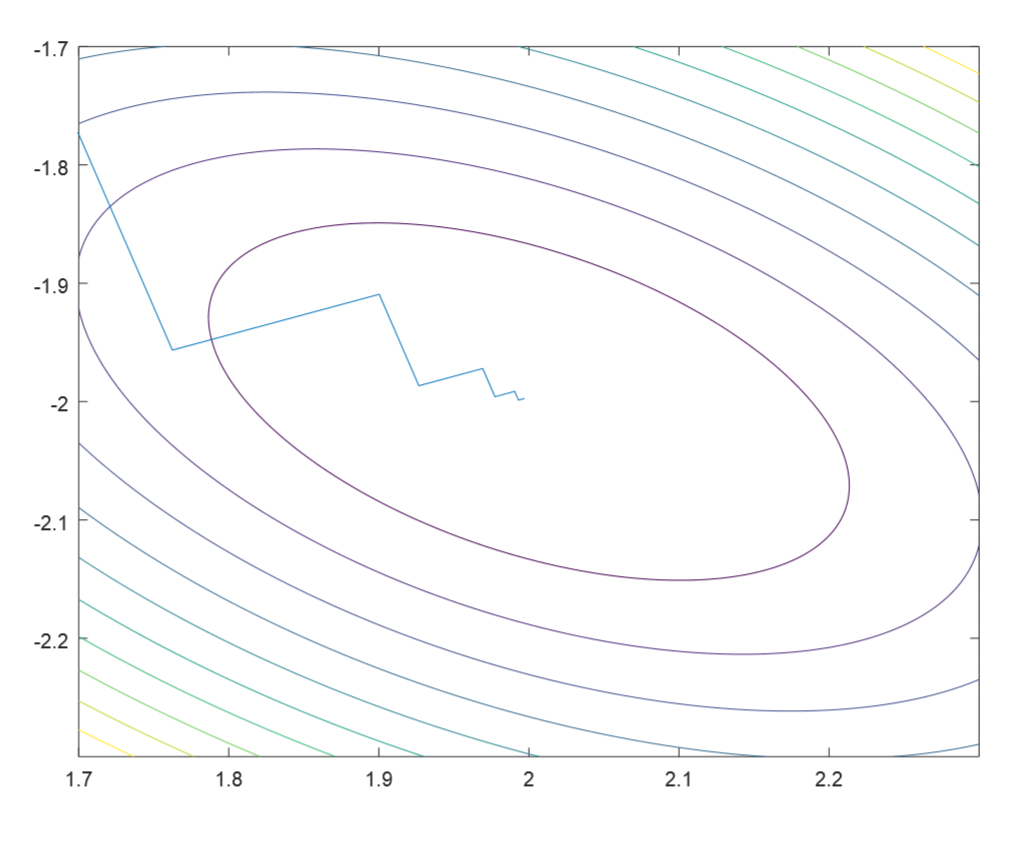
\includegraphics[scale=0.5]{AlfioQuarteroni/Victor.png} 
\end{center}

De acuerdo a la gráfica, el Método del Gradiente converge a la solución que está en $(2,-2)$ y es el mínimos de la función cuadrática $\Phi(x)$\\

%==============================================================================================================
%==============================================================================================================
% Para el grupo de Laura
%==============================================================================================================
%==============================================================================================================

Considerando el sistema lineal
$$ Ax=b$$
$$ A=\begin{pmatrix}
     3 &  2 \\
     2 &  6 \\
    \end{pmatrix}\ $$
    
$$ b=\begin{pmatrix}
     2 \\
     -8 \\
    \end{pmatrix}\ $$
    
Escribe la función $ \Phi(x) $ y muestre una interpretación gráfica de la solución de dicho sistema lineal. Pruebe algunas iteraciones del Método del Gradiente después de probar su convergencia.\\

\textbf{Solución:}

El Método del Gradiente converge para el caso debido a que es una matriz simétrica positiva. Esto es porque sus autovalores son positivos ($ \lambda_1=2, \lambda_2=7$).

Considerando un valor inicial 
$$x_0 = \begin{pmatrix}
     15 \\
     -13 \\
    \end{pmatrix}\ $$
Podemos mostrar en la siguiente tabla los valores del los vectores en cada iteración

\begin{table}[h]
    \centering
    \begin{tabular}{|r|l|l|}
        Iteración & $x$ &    $y$   \\
        \hline
         0  &  -11  &  -9 \\
         1  & -3.2124 & 0.99158 \\
         2  & 1.1873 & -2.43762 \\
         3  & 1.6741 & -1.81298 \\
         4  & 1.9492 & -2.02736 \\
         5  & 1.9796 & -1.98831 \\
         6  & 1.9968 & -2.00171 \\
         7  & 1.9987 & -1.99927\\
    \end{tabular}
\end{table}

\begin{center}
    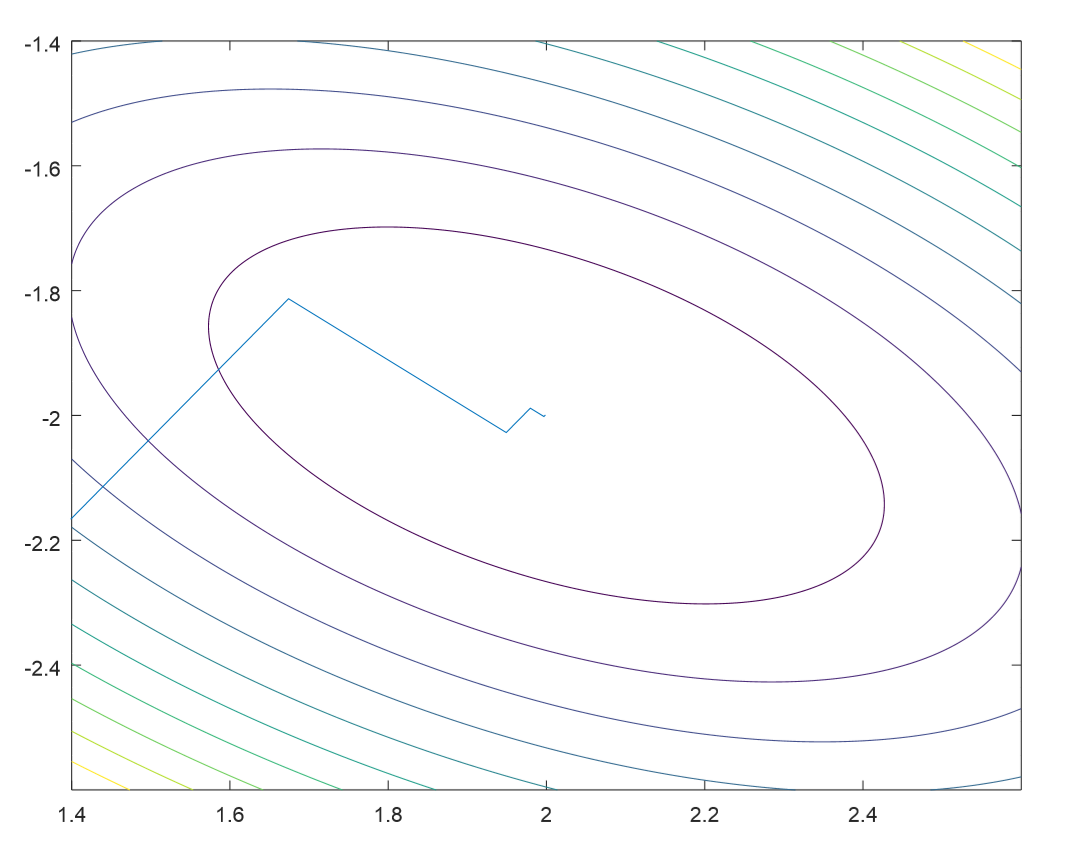
\includegraphics[scale=0.5]{AlfioQuarteroni/Laura.png} 
\end{center} 

De acuerdo a la gráfica, el Método del Gradiente converge a la solución que está en $(2,-2)$ y es el mínimos de la función cuadrática $\Phi(x)$\\